%!TEX root = ../notas_de_clase.tex


\chapter{Repaso de Probabilidades}

Este capítulo contiene un breve repaso sobre conceptos claves en la teoría de probabilidad, los cuales deben ser dominados para entender los contenidos del curso. Además, se hará una introducción a la teoría de la información, dando definiciones y teoremas claves de esta.

\section{Notación y conceptos básicos}

\subsection{Espacio de probabilidad}

Sea $\Omega$ un conjunto cualquiera, se considera a $\mathcal{P}(\Omega)$ el conjunto potencia de $\Omega$ dado por $\mathcal{P}(\Omega)=\{A:A\subseteq \Omega\}$, es decir, el conjunto de todos los subconjuntos de $\Omega$. Notar que el conjunto  vacío $\{\}=\phi$ siempre es un elemento en $\mathcal{P}(\Omega)$. También nos referimos a $\mathcal{P}(\Omega)$ como "las partes de $\Omega$."

\begin{definition}[$\sigma-$álgebra] Una $\sigma-$álgebra es un subconjunto $\Sigma\subseteq\mathcal{P}(\Omega)$ con las siguientes propiedades:
\begin{enumerate}
    \item $\Omega\in\Sigma$, $\phi\in\Sigma$,
    \item Si $A\in\Sigma$, entonces $A^{c}\in\Sigma$,
    \item Si $\{A_i\}_{i\in\mathbb{N}}\subseteq \Sigma$, entonces $\bigcup\limits_{i\in\mathbb{N}}A_i\in\Sigma$.
\end{enumerate}
\end{definition}

En adelante, se considera a $\Sigma$ una $\sigma-$álgebra sobre $\Omega$. Además, a la dupla $(\Omega, \Sigma)$ se le denomina \emph{espacio medible}. 

\begin{definition}[Medida]
Se dice que una función $\mu:\Sigma\rightarrow\R$ es una medida sobre $\Sigma$ si es que $\mu$ cumple que:

\begin{enumerate}
    \item Positividad: $\forall A \in\Sigma$, $\mu(A)\geq 0$,
    \item $\mu(\phi)=0$,
    \item $\sigma$-aditividad: Si $\{A_i\}_{i\in\mathbb{N}}$ es un conjunto disjunto, es decir, que $A_i\cap A_j=\phi, \forall i\neq j$, entonces:
    \[\mu\left( \bigcup\limits_{i\in\mathbb{N}}A_i \right)=\sum_{i\in\mathbb{N}}\mu(A_i).\]
    
\end{enumerate}
En el caso $\mu(\Omega)=1$, $\mu$ es una \emph{medida de probabilidad}.
\end{definition}

Antes de introducir lo que entenderemos como espacio de probabilidad, es necesario entender lo que es la $\sigma$-álgebra de Borel. Para esto, necesitamos la siguiente definición:

\begin{definition}[$\sigma$-álgebra generada por un conjunto]
Sea $\mathcal{L}\subseteq\mathcal{P}(\Omega)$ una familia de partes de $\Omega$. Consideremos a $\mathcal{J}$ como $\mathcal{J}(\mathcal{L})=\{\mathcal{B}:\mathcal{B}\text{ es $\sigma$-álgebra en }\Omega, \mathcal{L}\subseteq\mathcal{B}\}$, es decir, $\mathcal{J}(\mathcal{L})$ es el conjunto de todas las $\sigma$-álgebras sobre $\Omega$ que contienen al conjunto $\mathcal{J}$. La $\sigma$-álgebra \emph{generada por un conjunto $\mathcal{L}$}, $\sigma(\mathcal{L})$ está dada por:

\[\sigma(\mathcal{L})=\bigcap\limits_{\mathcal{B}\in\mathcal{J}}\mathcal{B}.\]
\end{definition}

 Basicamente, $\sigma(\mathcal{L})$ se entiende como la \emph{$\sigma$-álgebra más pequeña que contiene a $\mathcal{L}$}. Es decir, si $\sigma_0$ es cualquier $\sigma-$álgebra que contiene a $\mathcal{L}$, entonces necesariamente $\sigma(\mathcal{L})\subseteq\sigma_0$. 

En el caso que $\Omega=\mathbb{R}$, se dotará de este espacio de una $\sigma$-álgebra especial, la $\sigma$-álgebra de los \emph{Borelianos}, la cual es clave en la teoría de probabilidades. Si se considera que $\mathcal{L}=\{(-\infty, x]:x\in\mathbb{\mathbb{R}}\}$, la $\sigma$-álgebra de Borel  $\sigma(\mathcal{L})$ se denotará por $\mathbb{B}(\mathbb{R})$ o simplemente por $\mathbb{B}$. A los elementos de $\mathbb{B}$ se le llaman los \emph{borelianos}.

Consideremos a $\mu$ una medida, a la tripleta $(\Omega, \Sigma, \mu)$ se le denomina espacio de medida, en el caso de que $\mu$ sea una medida de probabilidad, entonces $(\Omega, \Sigma, \mu)$ es un espacio de probabilidad. En un espacio de probabilidad, a los elementos $\omega\in\Omega$ se le denominan eventos. Se denotará a las medidas de probabilidad como $\mathbb{P}$.  

\subsection{Propiedades de un espacio de probabilidad}

Consideremos a $(\Omega, \Sigma, \mathbb{P})$ un espacio de probabilidad y a $A,B\in\Sigma$. Se verifican las siguientes propiedades:

\begin{enumerate}
    \item Se cumple que $\PP (B\backslash A)=\PP (B)-\PP (B\cap A)$.
    \item $\PP$ es creciente, esto es:
    \[A\subseteq B \implies \PP (A)\leq \PP (B).\]
    \item $\PP (A^c)=1-\PP(A)$.
    \item $\PP(A\cup B)=\PP(A)+\PP(B)-\PP(A\cap B)$.
\end{enumerate}

\subsection{Probabilidad condicional}

En adelante, se considera a $(\Omega, \Sigma, \mathbb{P})$ un espacio de probabilidad fijo.

\begin{definition}
Sean $A,B\in\Sigma$ con $\PP (B)>0$. La probabilidad condicional de $A$ dado $B$ es:

\[\PP (A|B)=\dfrac{\PP (A\cap B)}{\PP(B)}.\]
\end{definition}

Es directo verificar las siguientes propiedades:

\begin{enumerate}
    \item Sean $A,B\in\Sigma$ con $\PP (A)>0$ y $\PP (B)>0$. Se tiene que:

\[\PP(A|B)=\dfrac{\PP(B|A)\PP(A)}{\PP(B)},\]

lo cual es conocido como el Teorema de Bayes.


\item Si $\{A_n:n\in\mathbb{N}\}\subseteq \Sigma$ es una familia disjunta, entonces se tiene que:

\[\PP\left(\bigcup\limits_{n\in\mathbb{N}}A_n|B\right)=\sum\limits_{n\in\mathbb{N}}\PP(A_n|B).\]
\end{enumerate}

\textcolor{blue}{Para más propiedades revisar: G.~Grimmett \& D.~Stirzaker, \emph{Probability and Random Processes}, Oxford Press, 2001.}


%\begin{prop}[Probabilidades totales]
 
%\end{prop}

%Por completar

\section{Teoría de la Información}

La teoría de la información es el estudio científico de las leyes matemáticas que rigen la transmisión y el procesamiento de la información, además de \emph{medir} la información y la representación de la misma. Esta teoría, tiene intersección con muchos campos, desde el lenguaje y criptografía, hasta las probabilidades. En esta sección, se introducirán conceptos y definiciones básicas de la teoría de la información, como la entropía y la información mutua. 


\subsection{Entropía}

Consideramos a $X$ e $Y$ dos variables aleatorias (VA) discretas con función de densidad $p_X$ y $q_Y$ y posibles valores $\mathcal{X}=x_1,x_2,...$ e $\mathcal{Y}=y_1,y_2,\ldots$. La Entropía de la VA $X$ se define de la siguiente forma:

\begin{align*}
    H(X)&=\mathbb{E}[-\log p_X]\\
    &=-\sum\limits_{n\geq 1}p_X(x_n)\log p_X(x_n).
\end{align*}

La entropía, en analogía a la termodinámica, es una medida de \emph{desorden} en los valores que puede tomar una VA, es decir, mientras menos predecible es el valor de la VA, mayor es su entropía. Se dice también que la Entropía es la cantidad de \emph{bits} necesarios para describir $X$. 

Se definen las entropías condicionales de $X$ dado $Y$ como:

\begin{align*}
    H(X|Y=y)&=-\sum\limits_{n}p_{x_n|y}\log (p_{X|Y}(x_n|y))\\
    H(X|Y)&=-\sum\limits_i\sum\limits_j p_{X,Y}(i,j)\log (p_{X|Y}(i|j)),
\end{align*}
se define análogamente a $H(X,Y)$, la entropía conjunta considerando la densidad conjunta $p_{X,Y}$.

\begin{prop}[Propiedades de la entropía]
Algunas propiedades de la entropía son las siguientes:

\begin{itemize}
    \item $0\leq H(X)\leq \log (|\mathcal{X}|)$,
    \item $0\leq H(X|Y)\leq H(X)$.
\end{itemize}

\end{prop}

\subsection{Información mutua}

La información mutua $I$ entre $X$ e $Y$ se define como:

\begin{align*}
    I(X;Y)&=H(X)-H(X|Y)\\
    &=\sum\limits_{i,j}p_{X,Y}(i,j)\log \dfrac{p_{X,Y}(i,j)}{p_X(i)p_Y(j)},
\end{align*}

la cual tiene las siguientes propiedades:

\begin{prop}[Propiedades Información Mutua]
Sean $X$ e $Y$ dos VAs, tenemos

\begin{enumerate}
    \item No negatividad: $I(X;Y)\geq 0$
    \item Simetría: $I(X;Y)=I(Y;X)$
    \item Regla de la cadena: $I(X;Y,Z)=I(X;Z)+I(X;Y|Z)$
\end{enumerate}

\end{prop}

\subsection{Relación entre Entropía e Información Mutua}

Algunas de las relaciones que existen entre la información mutua y la entropía son las siguientes:

\begin{align*}
    I(X;Y)&= H(X)-H(X|Y)\\
    &= H(Y)-H(Y|X)\\
    &= H(X)+H(Y)-H(X,Y)\\
    &= H(X,Y)-H(Y|X)-H(X|Y)
\end{align*}

las cuales, visualmente se obtienen dadas la figura \ref{fig:relationentropy}.

\begin{figure}[ht]
    \centering
    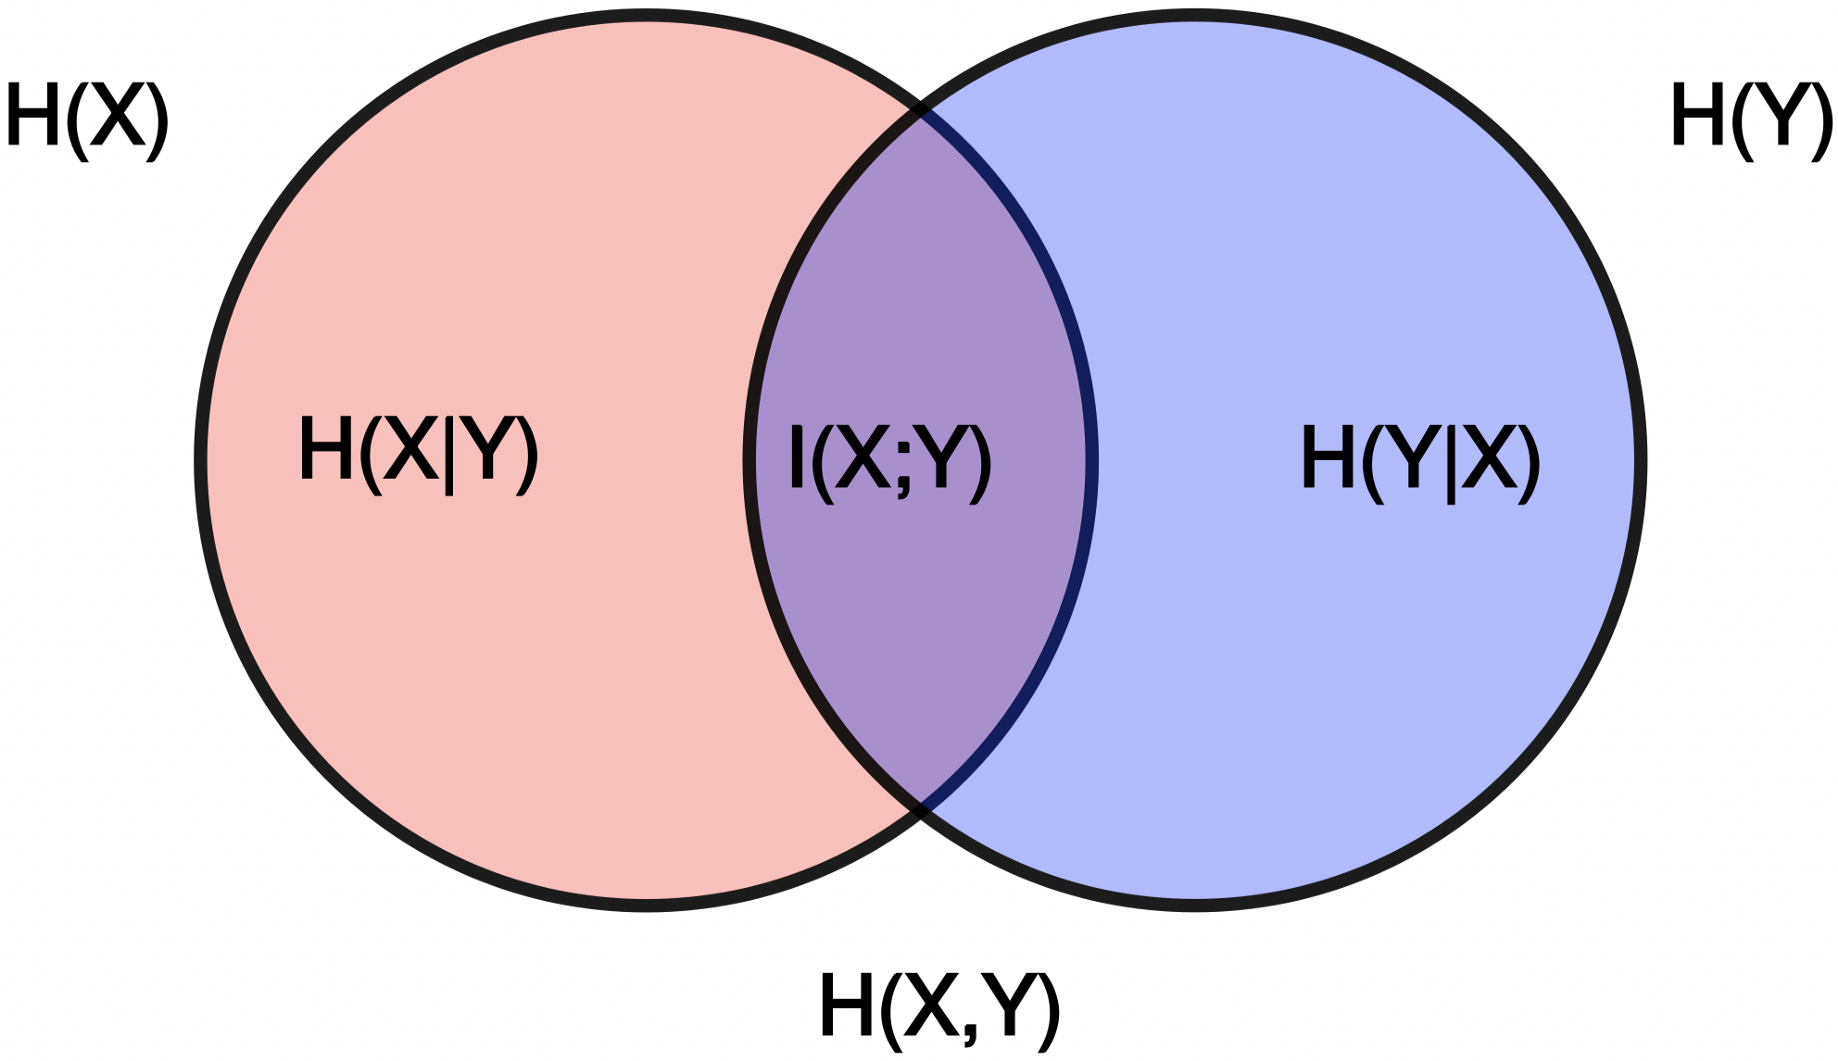
\includegraphics[width=0.7\columnwidth]{img/relationentropy.png}
    \caption{Relación entre $H$ e $I$}
    \label{fig:relationentropy}
\end{figure}

\subsection{Divergencia de Kullback-Leibler}

\begin{definition}[Divergencia de Kullback-Liebler]
Para dos densidades de probabilidad $f$ y $g$, definidas sobre un mismo conjunto de partida $\cX$, la divergencia de Kullback-Leibler entre ellas está definida mediante 
\begin{equation}
	\KL{f}{g} = \int_\cX f(x)\loga{\frac{f(x)}{g(x)}}\dx.
\end{equation}
\end{definition}

\begin{remark} La divergencia KL es siempre positiva $\forall f,g$ (desigualdad de Gibbs):
\begin{align*}
 	-\KL{f}{g}  &= \int_\cX f(x)\loga{\frac{g(x)}{f(x)}}\dx\\
 				&\leq \loga{\int_\cX f(x)\frac{g(x)}{f(x)}}\dx, \quad\quad \text{(Jensen's)}\\
 				&= \loga{\int_\cX g(x)}\dx\\
 				&=\log 1=0.,	
 \end{align*} 
Además, como $\log(\cdot)$ es estrictamente convexo, la igualdad $\KL{f}{g}=0$ solo se cumple si el argumento $\frac{g(x)}{f(x)}$ es constante, lo cual se tiene solo para ${g(x)} = {f(x)}$.
\end{remark}

Otra propiedad clave de la divergencia KL es que puede ser infinita y es asimétrica, por esta razón nos referimos a KL como divergencia y no \emph{distancia}. La intuición detrás de la KL es que es una medida de \textit{error} de estimar la densidad $f$ mediante la densidad $g$. Algunas propiedades son las siguientes:

\begin{prop}
\begin{enumerate}
    \item Relación con la información mutua:
    \[I(X;Y)=KL(p_{X,Y}||p_X p_Y)\]
\end{enumerate}
\end{prop}


\subsection{Data Processing Inequality}

\begin{theorem}[Data Processing Inequality (DPI)]
Sea una cadena de markov dada por las variables aleatorias $X\rightarrow Y\rightarrow Z$, se tiene que:

\[I(X;Y)\geq I(X;Z)\]
la cual se llama Data Processing Inequality (DPI), con igualdad si y solo si $X\rightarrow Z\rightarrow Y$ es una cadena de Markov. Esta desigualdad establece que no es posible realizar ningún procesamiento $Z$, determinístico o estocástico, que uno puede hacer a los datos $Y$ que puedan extraer más información sobre $X$ que la contenida inicialmente en los datos $Y$. 
\end{theorem}

Como corolario directo de la DPI, se tiene que para cualquier función determinista $g(\cdot)$ se cumple que:

\[I(X;Y)\geq I(X;g(Y))\]

y entonces no existe ninguna función de $Y$ la cual pueda aumentar la información que $Y$ contiene sobre $X$.



%\section{Modelos estadísticos de una muestra}

\section{Construcción de variables aleatorias mediante transformaciones}

\subsection{Chi-Cuadrado}

Sean $Z_1,\ldots, Z_n$ variables aleatorias $Z_i\sim\mathcal{N}(0,1)$ independientes, se tiene que la suma de sus cuadrados 
\[Q=\sum\limits_{i=1}^{n} Z_i^2,\]
distribuye según una distribución \textit{Chi-Cuadrado} con $n$ grados de libertad. Esto lo denotamos como:

\[Q\sim\mathcal{X}^2_n. \]
Algunas propiedades de esta distribución son:
\begin{enumerate}
    \item [a.] $\mathbb{E}(\mathcal{X}^2_n) = n$
    \item [b.] $\mathbb{V}(\mathcal{X}^2_n) = 2n$
    \item [c.] $M_{\mathcal{X}^2_n}(t) = (1-2t)^{\frac{-n}{2}}$ con $t<\frac{1}{2}$.
    
\end{enumerate}

\subsection{T-Student}

Sea $X_1,...,X_n$ una muestra i.i.d de una variable aleatoria $X\sim\mathcal{N}(\mu,\sigma^2)$. Consideremos el promedio muestral:
\[\overline{X}_n=\dfrac{1}{n}\sum\limits_{i=1}^n X_i,\]
y la varianza muestral insesgada:
\[S^2=\dfrac{1}{n-1}\sum\limits_{i=1}^n (X_i-\overline{X}_n)^2.\]

Entonces:
\[\dfrac{\overline{X}_n-\mu}{S/\sqrt{n}}\sim t_{n-1},\]
siendo $t_{n-1}$ la distribución t-student con $n-1$ grados de libertad.